\documentclass{beamer}
\mode<presentation>{
  \usetheme{boxes}
}


\usepackage[T1]{fontenc}
\usepackage[utf8]{inputenc}
\usepackage[swedish]{babel}
\usepackage{epstopdf}
\usepackage{array}

\usepackage{listings}
\usepackage{tikz}
\usetikzlibrary{trees,arrows,automata}

\usepackage{wasysym}
\usepackage{fancyvrb}
\DefineVerbatimEnvironment{code}{Verbatim}{fontsize=\small}
\DefineVerbatimEnvironment{example}{Verbatim}{fontsize=\small}
\newcommand{\ignore}[1]{
}

\lstnewenvironment{codeEx}
{\lstset{ basicstyle= \ttfamily }}
{}

\lstnewenvironment{codeExDiff}
{\lstset{ basicstyle=\color{black} \ttfamily
        , moredelim=[is][\color{red}]{|}{|}
        } }
{}


\newcommand{\ndist}{1.7cm}
\newcommand{\nshift}{0.6cm}
\newcommand{\nshiftw}{0.9cm}
\newcommand{\ncol}{blue!20!white}

\newcommand{\tree}[5] {
\begin{figure}[H]
    \centering
        \begin{tikzpicture}[->,node distance=\ndist, semithick]
            \tikzstyle{every state}=[fill=red!20!white,text=black]
            \node[state,fill=\ncol](add) {#2};
            \node[state,fill=\ncol](mul)[below of=add, xshift=\nshiftw] {#3};
            \node[state,fill=\ncol](sin)[below of=add, xshift=-\nshiftw] {#1};
            \node[state](x1)  [below of=sin, xshift=0cm] {#4};
            \node[state](x2)  [below of=mul, xshift=-\nshift]  {#4};
            \node[state](five)[below of=mul, xshift=\nshift]  {#5};
            \path (add) edge node {} (mul)
                        edge node {} (sin)
                  (mul) edge node {} (x2)
                        edge node {} (five)
                  (sin) edge node {} (x1);
        \end{tikzpicture}
\end{figure}

}




\begin{document}

\title{Optimering under körningstid}


\author{Simon Edwardsson\smiley \and Olle Fredriksson\smiley
\and \linebreak{}
Daniel Gustafsson\smiley \and Dan Rosén\frownie}


\institute{\smiley Chalmers Tekniska Högskola\and \frownie Göteborgs Universitet}

\everymath{\displaystyle}

\begin{frame}
    \titlepage
\end{frame}


\begin{frame}

[sin(x) * x] [Draw!]

\end{frame}

\begin{frame}[fragile]
\centering
\begin{tabular}{ m{2.4cm} m{0.5cm} m{5cm} }
    sin(x) + x * 5 & \pause $\Rightarrow$
    &
	\tree{sin}{+}{*}{x}{5}
\\
\end{tabular}
\end{frame}

\begin{frame}[fragile]
\centering
\begin{tabular}{ m{2.4cm} m{0.5cm} m{5cm} }
    sin(x) + x * 5 & $\Rightarrow$
    &
	\tree{Sin}{Add}{Mul}{Var}{Num}
\\
\end{tabular}
\end{frame}

\begin{frame}[fragile]
\centering
\begin{tabular}{ m{10cm} }
\tree{Sin}{Add}{Mul}{Var}{Num} \\
\begin{codeEx}
eval :: Expr -> Double -> Double
eval Var       x = x
eval (Num i)   x = i
eval (Add l r) x = eval l x + eval r x 
eval (Mul l r) x = eval l x * eval r x
\end{codeEx}
\\
\end{tabular}
\end{frame}

\begin{frame}[fragile]

Bild på en graf, där vi visar att det finns många olika x värden. Här säger vi också att det finns ett problem.
\begin{codeEx}
map (eval expr) [-10..10]
\end{codeEx}

\end{frame}

\begin{frame}[fragile] 
\centering
\begin{codeExDiff}
map (|optimise| (eval expr)) [-10..10]
\end{codeExDiff}

\pause

\begin{codeEx}
eval' x = sin x + x * 5
\end{codeEx}

\pause

\begin{codeExDiff}
map |eval'| [-10..10]
\end{codeExDiff}
\end{frame}

\begin{frame}
\centering
	\Huge{Demo}

\end{frame}


% knyta an till f;rra presentationen utan att utesluta de nya, kort namna att vi optimerar saker och forklarar ett vi nu ska ge ett exempel dar det ar anvandbart


\begin{frame}

	Vad sysslar vi egentligen med (vart befinner vi oss) (graf fran olle)

\end{frame}

\begin{frame}[fragile]
	Vad har hant sen sist?
	\pause
	Callstack
		Cool bild, forklarning
	\pause 
	Lathet, ge if exempel.

\begin{codeEx}
fact x = if (x == 0) 
    then 1
    else x * fact (x-1)
\end{codeEx}

\end{frame}

\begin{frame}
	Användningsområden.
\begin{itemize}
	\item Regular expressions
	\item Vetenskapliga beräkningar % dotproduct, power, newtonraphson, simuleringar
	\item Raytracer
\end{itemize}

Bild pa t ex newtonraphson kurva, nollpunkter och sant.

\end{frame}

\begin{frame}
	Focusera pa raytracer med resultat och bild pa alien.
	Fin bild.

\begin{figure}[H]
\centering
    
\includegraphics[width=0.3\textwidth]{img/shapes.png} 
\end{figure}


\end{frame}
\begin{frame}
\begin{figure}[H]
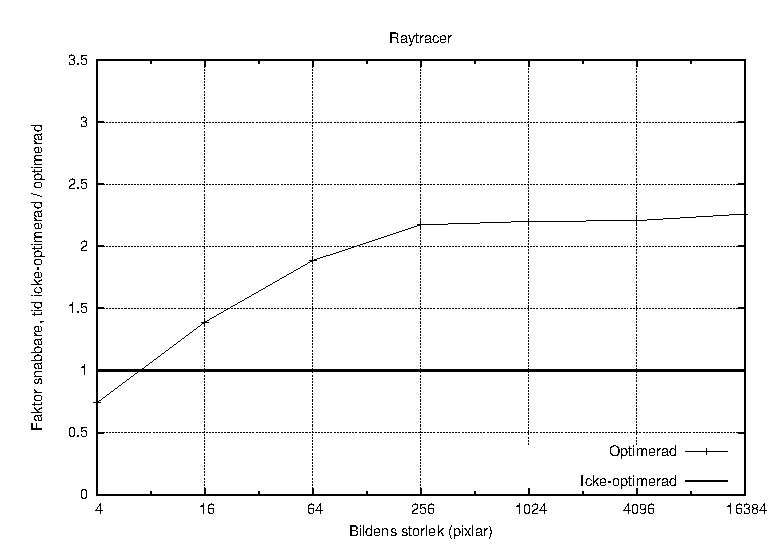
\includegraphics[width=1\textwidth]{shapesnormnocb.eps}
\end{figure}


\end{frame}

\begin{frame}

	Lardomar, reflextioner

\end{frame}

\begin{frame}
	Begransningar 
	Sharing. Rec	
\end{frame} 

\begin{frame}
	Framtida arbeten?
	Mycket pepp!
	Riktig kompilator
	Olles bild del 3.
	
	$\ddot\smile$ 
\end{frame}




\begin{frame}
\newcommand{\haskellcol}{red!20!white}
\newcommand{\ourcol}    {blue!20!white}
\newcommand{\stgcol}    {purple!20!white}
\newcommand{\runcol}    {green!20!white}
\begin{figure}[H]
        \begin{tikzpicture}[scale=0.5,transform shape,->,rounded corners
                           ,auto,node distance=3.2cm, semithick]
        \tikzstyle{every state}=[fill=\haskellcol
                                ,rectangle
                                ,minimum size=2.0cm]
        \node<5->[state](haskell)[above of=stg]                   {Haskell};
        \node<1->[state,fill=\stgcol](stg)    []                   {STG-kod};
        \node<2->[state,fill=\ourcol](socker) [left of=stg]        {Sockerkod};
        \node<3->[state,fill=\runcol](int) [right of=stg,xshift=3.0cm] {
          \begin{tikzpicture}[semithick]
            \node<3->[state,fill=\ourcol](stgint) [right of=stg]       {STG-tolk};
            \node<4->[state,fill=\ourcol](opt)    [right of=stgint]    {Optimering};
            \path<4->
              (stgint) edge[bend left] node {} (opt)
              (opt)    edge[bend left] node {} (stgint);
          \end{tikzpicture}
          Körning
        };
        \node<6->[state](comp)   [below of=stg]       {Kompilering \& optimering};
        \node<7->[state,fill=\runcol](run)    [below of=comp]      {
          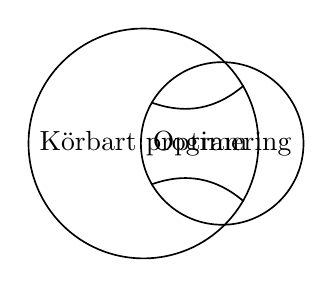
\begin{tikzpicture}[semithick]
            \node<7->[state](runinner) [] {Körbart program};
            \node<8->[state](optcomp)  [right of=runinner] {Optimering};
            \path<8->
              (runinner) edge[bend left] node {} (optcomp)
              (optcomp)  edge[bend left] node {} (runinner);
          \end{tikzpicture}
          Körning
        };
        \path<2-> (socker) edge            node {} (stg);
        \path<3-> (stg)    edge            node {} (int);
        \path<6-> (stg)    edge            node {} (comp);
        \path<5-> (haskell) edge           node {} (stg);
        \path<7-> (comp)   edge            node {} (run);
        \end{tikzpicture}
    \caption{Översikt}
    \label{figure:overviewSugar}
\end{figure}
\end{frame}

\end{document}
